\documentclass[12pt]{article}
\pdfoutput=1 

\addtolength{\oddsidemargin}{-.875in}
\addtolength{\evensidemargin}{-.875in}
\addtolength{\textwidth}{1.75in}

\addtolength{\topmargin}{-.875in}
\addtolength{\textheight}{1.75in}

\openup 1em

%macro for commenting
\usepackage{color}
\newcommand{\leo}[1]{{\color{blue}{\it leo: #1}}}
\newcommand{\xbeta}{\boldsymbol X_i^T \boldsymbol\beta}


\usepackage[round]{natbib}

\usepackage{rotating}
\usepackage{graphicx}
\usepackage{subcaption}

\usepackage{float}

\usepackage{amsthm,amsmath} 
\usepackage{amssymb}
\usepackage{subcaption}
\captionsetup{compatibility=false}

\usepackage[utf8]{inputenc}
\usepackage{algorithm}
\usepackage[noend]{algpseudocode}


\newtheorem{theorem}{Theorem}
\newtheorem{corollary}{Corollary}

\thispagestyle{empty}
\baselineskip=28pt

\title
    {One-Hot Membership Model}


\date{}

\begin{document}
    
\maketitle

\section{Introduction}

hard clustering:
several overly strong assumptions in k-means

soft clustering:
large variance induced by way too many non-zeros in the probability simplex.

\section{One-Hot Membership Model}

\subsection{General Framework}

Let $y_i$ be the observed data following the distribution $F$ with parameter $\theta_i$. Consider a  membership model with $\kappa$ possible membership:

\begin{equation}
\begin{aligned}
& \pi(y_i) \stackrel{indep}{\sim} F(y_i|\theta_i) \\
& \pi(\theta_i) = \sum_{k=1}^{\kappa} z_{k,i} \delta_{\theta^*_{k}}(\theta_i) \\
\end{aligned}
\label{membership_model}
\end{equation}
where $\{ z_{.,i}\}$ denotes the membership with only one $1$ and $(k-1)$ many $0$'s.

To allow borrowing of strength among $\{ z_{.,i}\}$, we assume $z_{.,i}$ follows:

\begin{equation}
\begin{aligned}
& \pi (z_{.,i}) \propto  \prod_{k=1}^{\kappa} (u_{k,i}v_{k} )^{z_{k,i}}  \\
 & v_{k} \sim Dir_{\kappa}(1,1,\ldots 1)\\
  & u_{.,i} \stackrel{iid}{\sim} Dir_{\kappa}(\epsilon,\epsilon,\ldots \epsilon)\\
\end{aligned}
\label{one_hot}
\end{equation}
where $\epsilon$ is a small number close to $0$, which causes $u_{k,i}$ to have only one value close to $1$ and the rest close to $0$. Due to the $z_{.,i}$ will take one-of-$\kappa$ memberships with probability almost $1$, we refer this  as one-hot membership model.

To compare with other methods, note when $\{z_{.,i}\}$ is assumed to be independent for each $i$, (\ref{membership_model}) is exactly the same as the k-means model; when $u_{k,i}$ is fixed to $1/\kappa$ for all $k,i$, the membership $z_{.,i}$ can be integrated out to obtain general finite mixture model.

The key difference is in one-hot membership model, the multinomial distribution of $z_{.,i}$ has its probability weight concentrated to one vertex, so that the estimate of $z_{.,i}$ is obtained via maximization, instead of expectation or sampling as in the general mixture model.
 
\subsection{Estimation}

\begin{equation}
\begin{aligned}
& \log[ \{y_i\}_i, \{z_{k,i}\}_{k,i} ] =  \sum_{i}\sum_{k=1}^{\kappa} z_{k,i} \log \{\delta_{\theta_{k}}(y_i) v_k \}
\end{aligned}
\label{conditional_lik}
\end{equation}

 This allows us to utilize Expectation-Maximization algorithm for parameter estimation:

\begin{algorithm}[H]
\caption{Estimation algorithm}\label{alg:euclid}
\begin{algorithmic}[1]
\While{$||\theta^{(s)}-\theta^{(s+1)}||>\epsilon$}%\Comment{We have the answer if r is 0}
\State Maximize over $\{ z_{i,k}\}_k$ by $ \underset{\{z_{i,k}\}_k} {\text{argmax }}\{z_{i,k}  v_{k}F (y_i|\theta^*_k)\}$ for all $i$;
\State Update $\theta^{*}_{k}= \text{argmax} \sum_{i=1}^{n} z_{k,i} \log F(y_i|\theta^*_k) $ for all $k$ 
\State Update $v_{k}=  \sum_{i} z_{k,i} /  \sum_{i}\sum_{k}z_{k,i}$ 
\EndWhile
\end{algorithmic}
\end{algorithm}

\section{Theory}


\subsection{Empirical Result: Bias-Variance Trade-off}

We generate data $y_i$ from $N(\mu_i, 0.5^2)$, using $75\%$ with $\mu_i =1$ and $25\%$ with $\mu_i =2$.

\begin{figure}[H]
\centering
\begin{subfigure}[t]{.8\columnwidth}
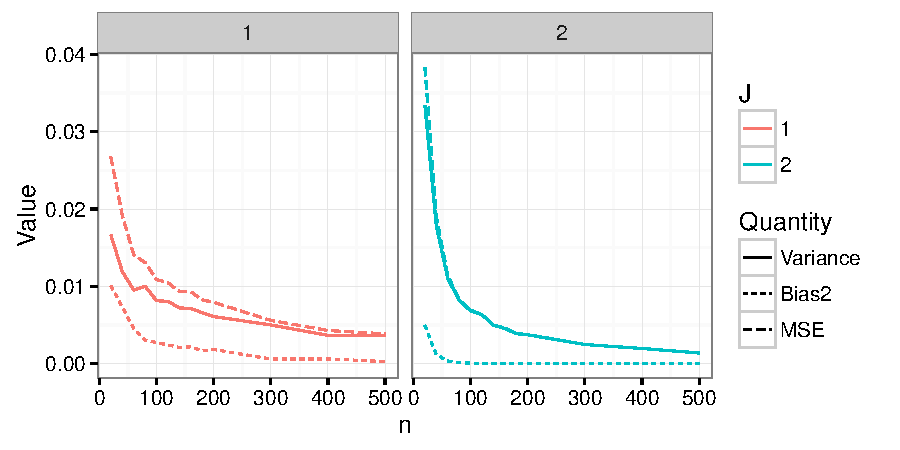
\includegraphics[width=\textwidth]{BV2.pdf}
\caption{The bias-variance trade-off.}
\end{subfigure}
\begin{subfigure}[t]{.8\columnwidth}
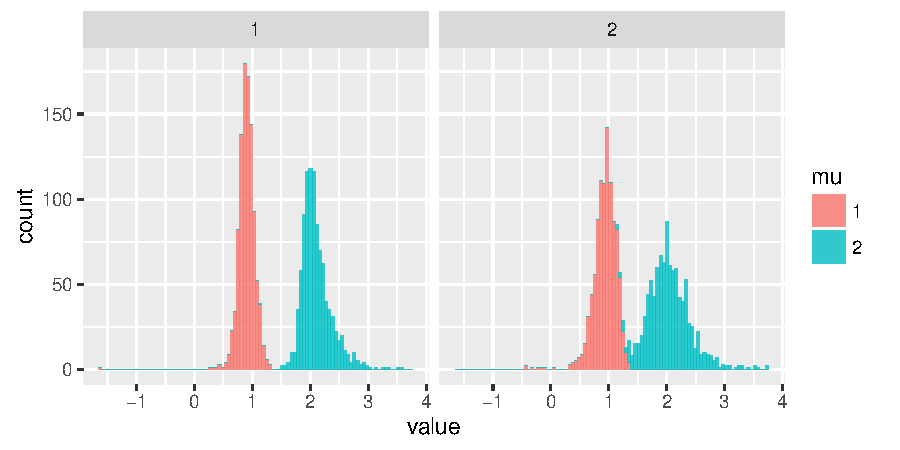
\includegraphics[width=\textwidth]{BVMeanDist.pdf}
\caption{The distribution of MLE for $\mu_1$ and $\mu_2$ over 1,000 simulation data sets, with total $40$ data points.}
\end{subfigure}
\begin{subfigure}[t]{.8\columnwidth}
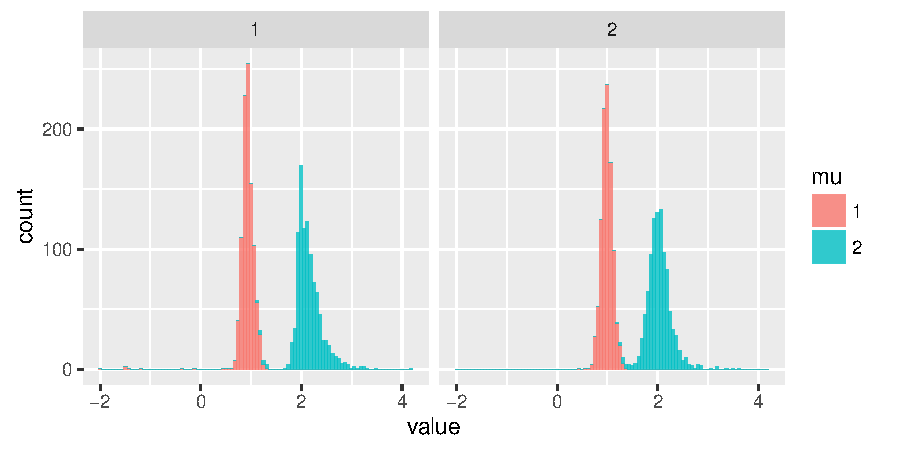
\includegraphics[width=\textwidth]{BVMeanDist3.pdf}
\caption{The distribution of MLE for $\mu_1$ and $\mu_2$ over 1,000 simulation data sets, with total $150$ data points.}
\end{subfigure}
\end{figure}

\subsection{Variance Reduction in Small Sample Size}

Let superscript denote the variable to be integrated over.
Using variance decomposition, the variance of the parameter estimator $\hat\theta$ has:

$$\mbox{Var}^{y} (\hat\theta) = \mbox{E}^{z}\mbox{Var}^{y} (\hat\theta| z) + \mbox{Var}^{z}\mbox{E}^{y} (\hat \theta| z)$$

Using subscript $FMM$ and $OH$ to denote the different models. As each $z_i$ is maximized to a fixed value in each dataset in one-hot model, It can be immediately seen that $\mbox{Var}_{OH}^{z}\mbox{E}^{y} (\hat \theta| z)=0$ and $\mbox{E}^{z}_{OH}\mbox{Var}^{y} (\hat\theta| z) = \mbox{Var}^{y}_{OH} (\hat\theta| z)$; whereas each $z_i$ is random in finite mixture model, $\mbox{Var}_{FMM}^{z}\mbox{E}^{y} (\hat \theta| z)\ge 0$. Therefore, it suffices to have $\mbox{Var}_{OH}^{y} (\hat\theta| z) - \mbox{E}^{z}\mbox{Var}^{y}_{FMM} (\hat\theta| z) < \mbox{Var}_{FMM}^{z}\mbox{E}^{y} (\hat \theta| z)$ for a reduction in variance.


\section{Simulation}




\section{Application}
\section{Discussion}

\bibliographystyle{plainnat}
\bibliography{reference}

\end{document}
